


\begin{figure*}[t]
    \centering
    % \vspace{-0.7cm}
    \vspace{3mm}
    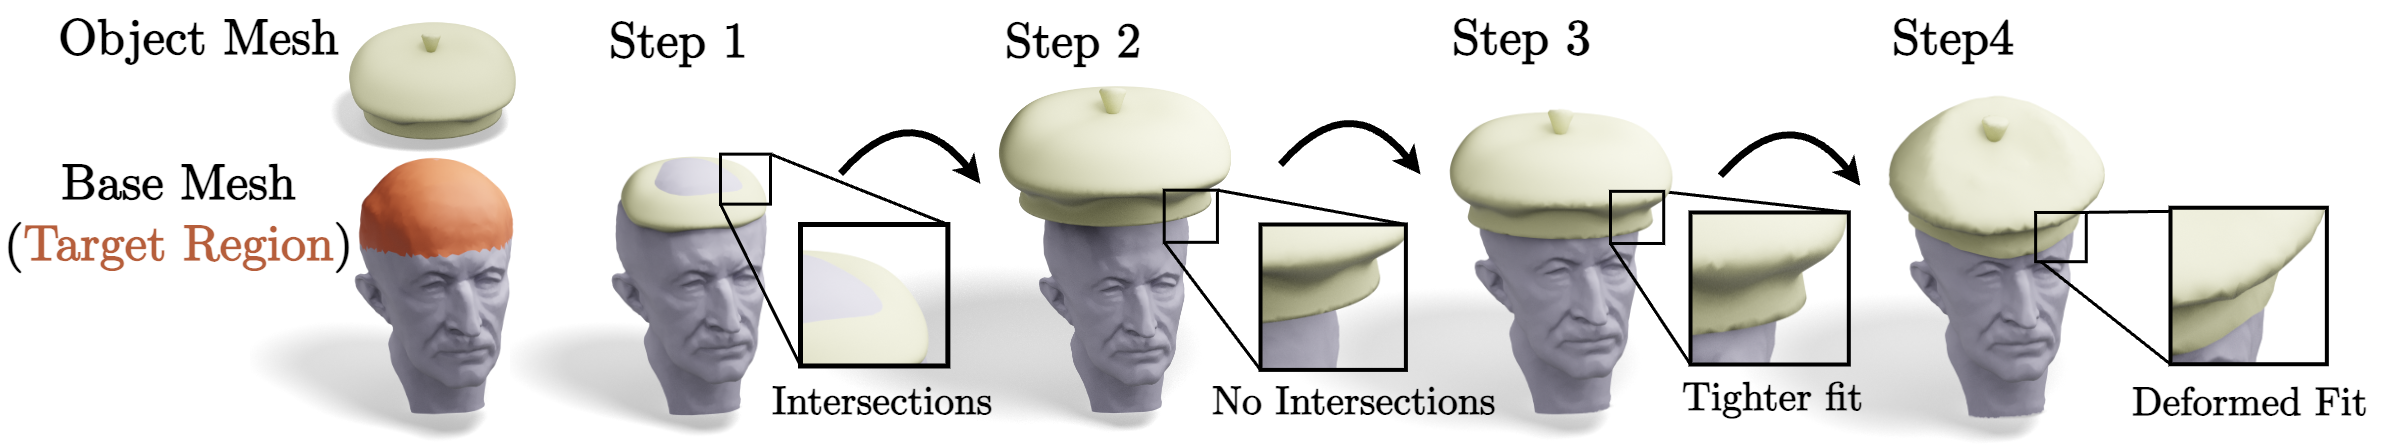
\includegraphics[width=\textwidth]{figures/main_method/main_method.png}   
    \caption{We compose the two meshes through a multi-step optimization pipeline: from an initialization obtained with a Vision-to-Language Model (\autoref{sec:initialization}), we start by obtaining a tight fit containing intersections (\autoref{sec:step1}), which we then resolve (\autoref{sec:step2}). After finetuning the fit to obtain the best possible rigid fit (\autoref{sec:step3}), we improve it further by allowing small deformations in the accessory object (\autoref{sec:step4}).}
    \label{fig:main_method}
    %\vspace{-2cm}
    \vspace{-3mm}
\end{figure*}

% \vspace{-6mm}
\section{Related Work} 

\label{sec:related_work}


\subsection{3D Registration}

The alignment of 3D objects is a fundamental problem in computer vision and graphics that has been studied thoroughly for decades \cite{mckay2003review,salvi2007survey, tam2013registration}. In this task, one seeks to find a transformation of an object to minimize an error metric defined with respect to another. A prominent work in this field is the Iterative Closest Point \cite{besl1992method,segal2009generalized}, which finds the optimal rotation and translation between two point clouds to minimize the distance between them. Among follow-up works to ICP are the globally optimal ICP (Go-ICP) \cite{yang2015go} and Fast Global Registration (FGR) \cite{zhou2016fast}.

In the deep learning era, numerous works have leveraged the power of neural networks for the registration problem, where the Euclidean distance between points has been replaced with the similarity of points in a learned feature space \cite{litany2017deep,aoki2019pointnetlk,wang2019dcp,huang2020fmr,choy2020dgr,lang2021dpc,yew2022regtr,jiang2023se}. Our mesh composition problem can be thought of as a registration problem between the asset mesh and the corresponding region on the body mesh. However, different from previous work that aligned two observations of the \textit{same} object, the asset is completely different from the target body region, making the problem highly challenging.

\subsection{Mesh Deformation}
A large body of research has been dedicated to surface deformation. Classical methods typically define an energy function subject to which the mesh is optimized, where the objective embodies desired properties of the deformed result \cite{yu2004poisson,botschsorkine08deformsurvey,skinningcourse:2014,Fulton:LSD:2018}. As-Rigid-As-Possible \cite{sorkine2007rigid} and Laplacian surface editing \cite{sorkine2004laplacian} are seminal works in this domain, which encourage smooth and rigid deformations. Such methods are applied to the subject mesh independently, without considering its interaction with other objects. 

% \itai{@someone, back me up on this independent claim, or refine as needed.}

In light of the unprecedented success of deep learning, researchers have incorporated deep foundation models as implicit guidance for the deformation process instead of the traditional hand-crafted optimization objective, leveraging the rich semantic priors embodied in these models and enjoying their intuitive language-based interface \cite{michel2022text2mesh,xu2024fusiondeformer,yang2024dreammesh,chen2024textmeshrefine}. TextDeformer \cite{michel2022text2mesh} used the CLIP model for deforming a source mesh toward a textual description, like turning a hand into an octopus. Follow-up works employed a powerful diffusion model for other deformation-driven creative applications, including concept blending \cite{kim2025meshup} and identity-preserving geometric stylization~ \cite{dinh2025geometry}. 

Similarly, we also leverage a diffusion model to guide the deformation of the accessory mesh. In contrast to prior work, the deformation in our case is constrained by the body mesh it should be composed onto, considering both their global semantic alignment and their local geometric fitting.

A recent work tackled the problem of designing creative 3D objects that fit a body mesh \cite{guo2025craft}. However, in stark contrast to our work, in CRAFT \cite{guo2025craft}, the contact points between the meshes are \textit{given} as input, while our method \textit{finds} the alignment between the meshes from a \textit{random initialization} of the asset object. 
%Additionally, the penetration avoidance between the asset and body is posed as a \textit{soft constraint}, while we \textit{guarantee} intersection-free composition of the meshes \textit{by construction}.

More relevant to our work is Instan3dit \cite{barda2025instant3dit}. In this work, the authors augment a base mesh with an accessory, such as adding a honey pot between the hands of a bear. The edit is implemented as a multi-view inpainting problem, followed by a 3D reconstruction from the posed images. While the results are visually appealing, the contact between the local edit and the body mesh is not modeled explicitly, leading to the gluing of the two. In our work, on the other hand, we consider the mesh interaction explicitly and successfully preserve the base and asset mesh properties (see \cref{fig:instant3dit_comparison}).

%\itai{I have a personal beef with this work. You might have to tone me down in this paragraph ha ha.}

%Additionally, the contact points and penetration avoidance between the asset and body are posed as \textit{soft constraints}


% \clearpage
